\chapter{Исследовательский раздел}

\section{Оценка алгоритмов}

В данном разделе будет проведено сравнение алгоритмов линейного и бинарного поиска по количеству сравнений, потребовавшихся для получения ответа. Длина массива равна $n = 1020$. 

Для алгоритма поиска полным перебором существует $n + 1$ возможных исходов: $n$ случаев расположения ключа в массиве и случай, когда ключ не найден. В худшем случае ключ может либо находиться в самом конце массива, либо отсутствовать вовсе, при этом количество сравнений в худшем случае будет равно $n$. В лучшем случае ключ будет находиться в начале массива и для его нахождения потребуется только одно сравнение. На рисунке~\ref{fig:linear_hist} представлена гистограмма, отображающая количество сравнений для каждого элемента в массиве при линейном поиске. Крайний правый и крайний левый столбцы гистограммы соответствуют худшим случаям.

\begin{figure}[H]
\centering
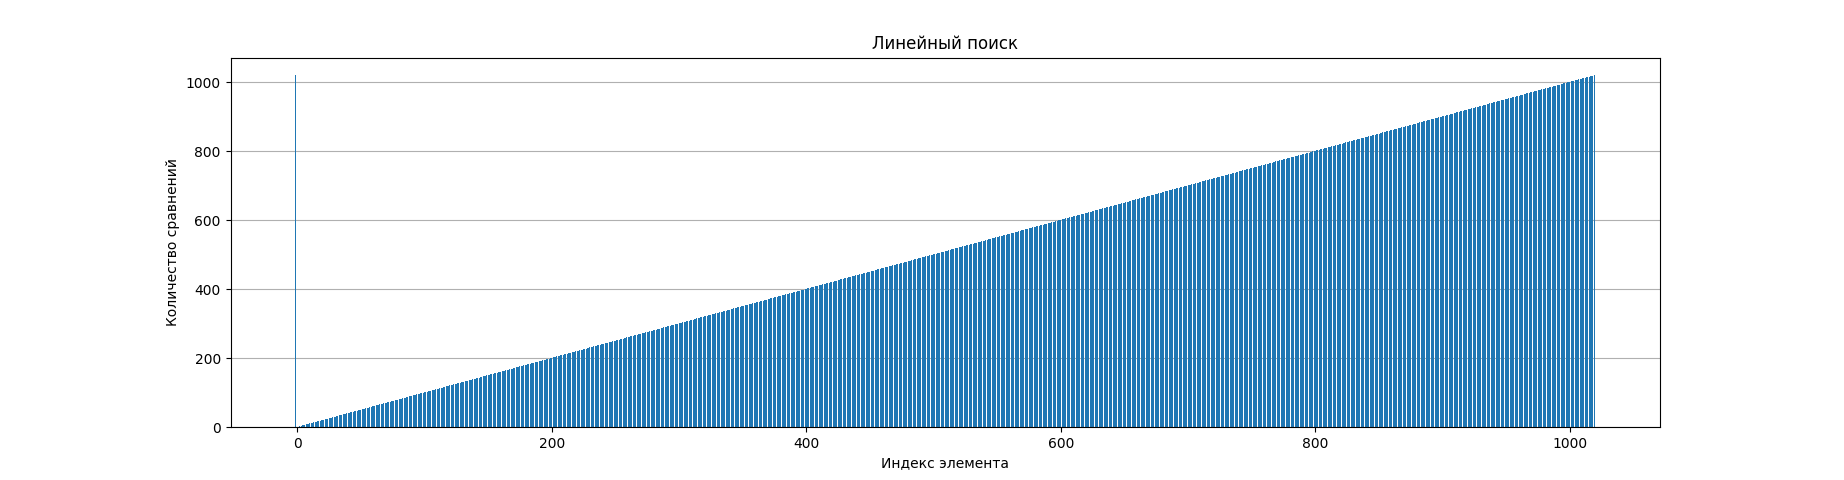
\includegraphics[width=\textwidth]{inc/img/linear_search_hist.png}
\caption{Количество сравнений для каждого элемента в массиве при линейном поиске}
\label{fig:linear_hist}
\end{figure}

На рисунке~\ref{fig:binary_hist} представлена гистограмма, отображающая количество сравнений для каждого элемента в массиве при бинарном поиске. Для алгоритма бинарного поиска количество сравнений в худшем случае не превышает $log_2(n)$.

\begin{figure}[H]
\centering
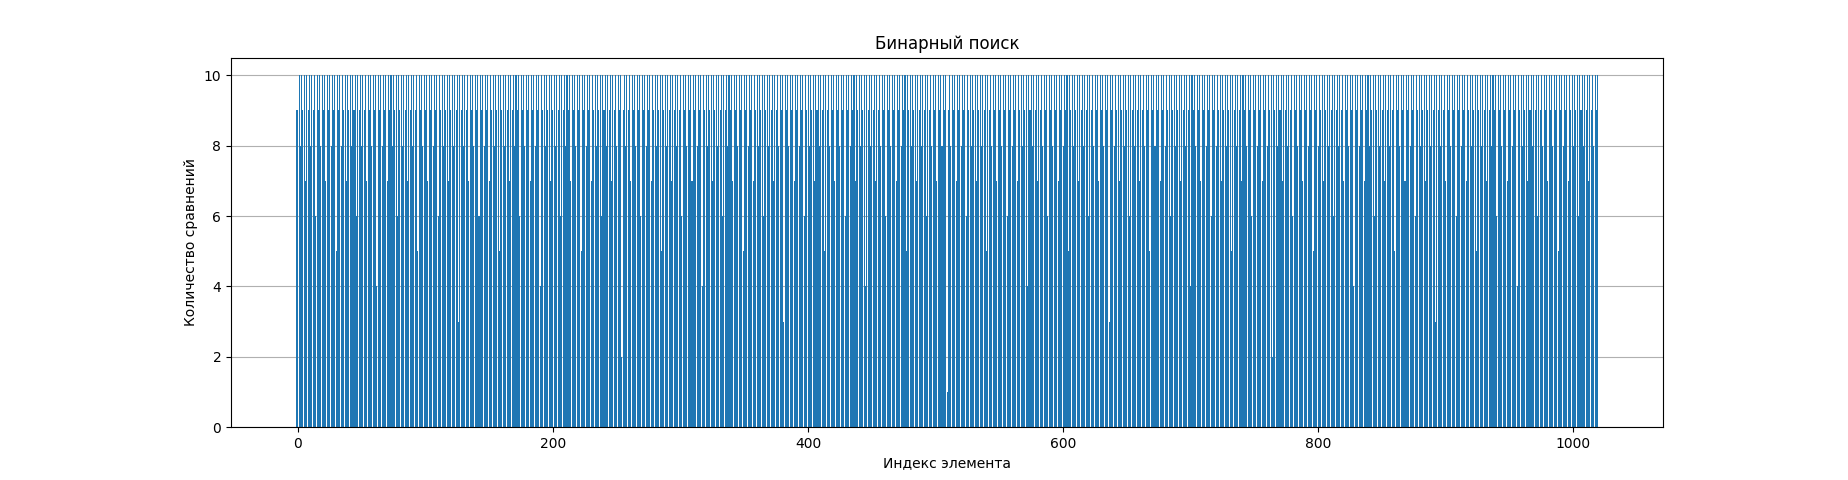
\includegraphics[width=\textwidth]{inc/img/binary_search_hist.png}
\caption{Количество сравнений для каждого элемента в массиве при бинарном поиске}
\label{fig:binary_hist}
\end{figure}

На рисунке~\ref{fig:binary_hist_sorted} представлена гистограмма, на которой элементы отсортированы по количеству сравнений при бинарном поиске. В таком случае количество сравнений под индексом $i$ ($i=\overline{0, n-1}$) соответствует максимальному количеству сравнений для массива длины $i+1$.

\begin{figure}[H]
\centering
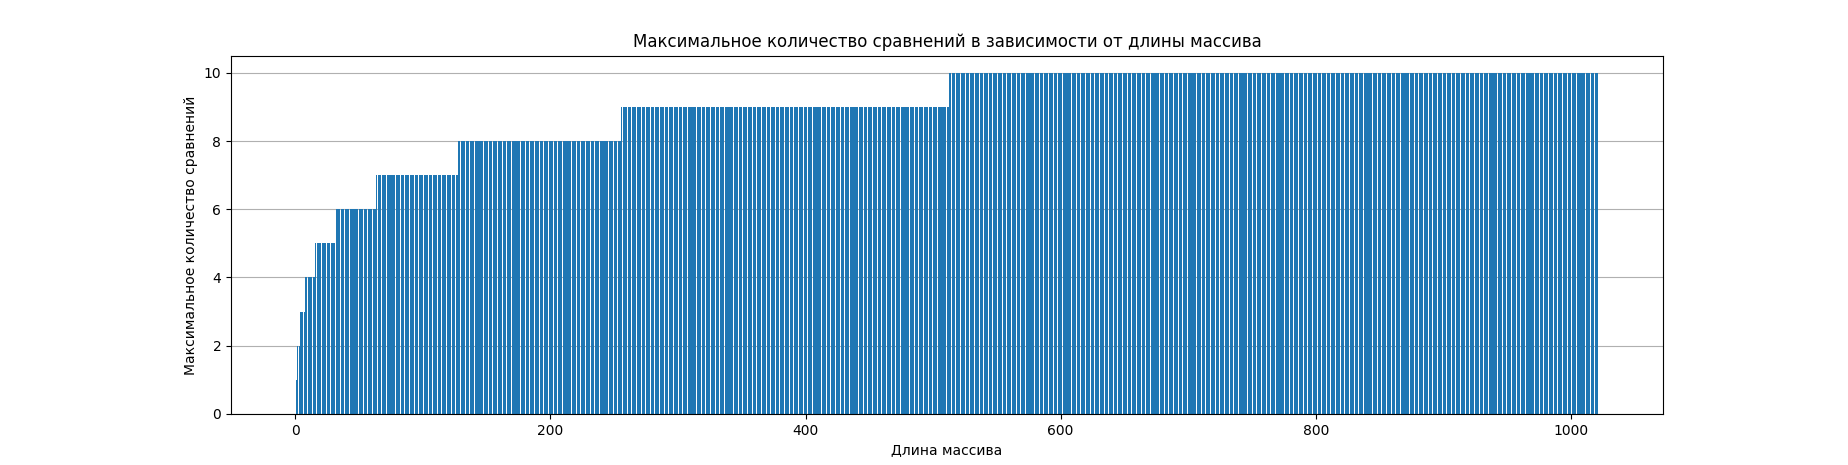
\includegraphics[width=\textwidth]{inc/img/binary_search_hist_sorted.png}
\caption{Максимальное количество сравнений при бинарном поиске в зависимости от длины массива}
\label{fig:binary_hist_sorted}
\end{figure}

На рисунке~\ref{fig:linear_vs_binary} представлены приближенные версии гистограмм, отображающих количество сравнений для каждого элемента при линейном и бинарном поиске на отсортированном массиве.

\begin{figure}[H]
    \centering
    \begin{minipage}[t]{0.48\textwidth}
        \centering
        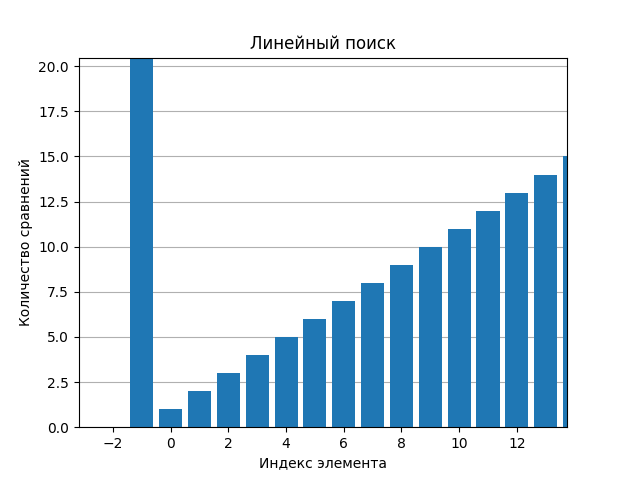
\includegraphics[width=\linewidth]{inc/img/linear_9.png}
        \caption*{а) Линейный поиск}
    \end{minipage}
    \hfill 
    \begin{minipage}[t]{0.48\textwidth}
        \centering
        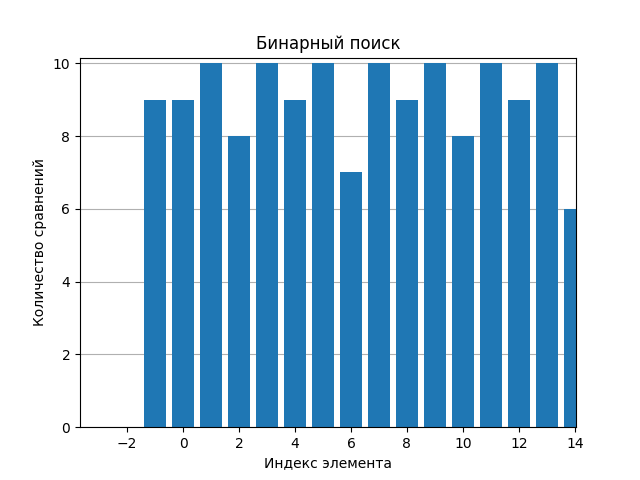
\includegraphics[width=\linewidth]{inc/img/binary_9.png}
        \caption*{б) Бинарный поиск}
    \end{minipage}

    \caption{Количество сравнений при линейном и бинарном поиске на отсортированном массиве}
    \label{fig:linear_vs_binary}
\end{figure}

В таблице~\ref{table:comparisons} продемонстрировано количество сравнений при линейном и бинарном поиске при индексах $i = \overline{0,10}$. Для индексов, меньших $log_2(1020)~\approx~9.994$, количество сравнений при линейном поиске меньше или равно количеству сравнений при бинарном поиске.

\begin{table}[htb]
\caption{Количество сравнений при линейном и бинарном поиске при индексах $i = \overline{0, 10}$}
\small
\centering\begin{tabular}{|c|c|c|c|}
        \hline
        \textbf{Индекс} & \textbf{Линейный поиск} & \textbf{Бинарный поиск} \\
        \hline
        0 & 1 & 9 \\
        \hline
        1 & 2 & 10 \\
        \hline
        2 & 3 & 8 \\
        \hline
        3 & 4 & 10 \\
        \hline
        4 & 5 & 9 \\
        \hline
        5 & 6 & 10 \\
        \hline
        6 & 7 & 7 \\
        \hline
        7 & 8 & 10 \\
        \hline
        8 & 9 & 9 \\
        \hline
        9 & 10 & 10 \\
        \hline
        10 & 11 & 8 \\
        \hline
    \end{tabular}
\label{table:comparisons}
\end{table}

\newpage
\section{Вывод}

При поиске заданного ключа в массиве полным перебором количество сравнений растёт линейно с увеличением индекса ключа. В случае, если массив отсортирован и для нахождения элемента используется бинарный поиск, то количество сравнений не будет превышать $log_2(n)$, где $n$ --- размер массива. Хотя скорость роста функции $log_2(n)$ меньше (при увеличении $n$), чем у функции $n$, для отсортированного массива количество сравнений при линейном поиске может быть меньше или равно количеству сравнений при бинарном поиске, если индекс искомого ключа меньше $log_2(n)$. В исходном массиве, длиной $n = 1020$, для элементов, расположенных по индексам $i = \overline{0, 9}$, количество сравнений при линейном поиске будет меньше или равно количеству сравнений при бинарном поиске.
